\documentclass[12pt]{article}
\usepackage[utf8]{inputenc}
\usepackage[spanish]{babel}
\usepackage{amsmath, amssymb}
\usepackage{graphicx}
\usepackage{float}
\usepackage{caption}
\usepackage{subcaption}
\usepackage{booktabs}
\usepackage{hyperref}
\usepackage{listings}
\usepackage{color}
\usepackage{geometry}
\geometry{margin=2.5cm}

\title{Trabajo Práctico 3 \\
Simulación de un modelo MM1 e Inventario}
\author{
    Renzo Aimaretti \\ \texttt{renzoceronueve@gmail.com}
    \and
    Facundo Sosa Bianciotto \\ \texttt{facundososabianciotto@gmail.com}
    \and
    Vittorio Maragliano \\ \texttt{maraglianovittorio@gmail.com}
    \and
    Ignacio Amelio Ortiz \\ \texttt{nameliortiz@gmail.com}
    \and
    Nicolás Roberto Escobar \\ \texttt{escobar.nicolas.isifrro@gmail.com}
    \and
    Juan Manuel De Elia \\ \texttt{juanmadeelia@gmail.com}
}
\date{\today}

% Configuración de código fuente Python
\definecolor{codegray}{gray}{0.95}
\lstset{
    backgroundcolor=\color{codegray},
    basicstyle=\ttfamily\footnotesize,
    frame=single,
    breaklines=true,
    language=Python
}

\begin{document}

\maketitle
\newpage

\begin{abstract}
Este informe presenta un estudio de simulación de dos modelos clásicos en teoría de colas y gestión de inventarios: el modelo M/M/1 y el modelo de inventario $(s, S)$. La simulación fue desarrollada en Python, con múltiples configuraciones paramétricas y análisis estadísticos. Además, se realizó una implementación paralela en AnyLogic para comparar resultados. Se incluyen las métricas principales de desempeño, sus gráficas correspondientes y una comparación con los valores teóricos esperados. El objetivo es validar el comportamiento de los modelos bajo distintas cargas del sistema o demandas, y analizar su eficiencia operativa y económica.
\end{abstract}

%-------------------------------------
\section{Introducción}
%-------------------------------------
\begin{itemize}
    \item Descripción general del objetivo del trabajo.
    \item Motivación de la simulación de modelos clásicos.
    \item Breve mención de las herramientas utilizadas: Python, AnyLogic, y calculadoras teóricas.
    \item Mención de que se compararán tres fuentes de resultados: teórico, Python, AnyLogic.
\end{itemize}

%===========================================================
\section{Modelo M/M/1}
%===========================================================

\subsection{Marco Teórico}

El modelo M/M/1 representa un sistema de colas con las siguientes características:

\begin{itemize}
    \item Llegadas de clientes según un proceso de Poisson con tasa $\lambda$.
    \item Tiempos de servicio con distribución exponencial de tasa $\mu$.
    \item Un solo servidor.
    \item Capacidad de la cola opcionalmente finita (tamaño máximo $K$).
    \item Los clientes que arriban y encuentran la cola llena son rechazados.
\end{itemize}

\textbf{Fórmulas teóricas para el caso de cola infinita:}

\begin{align*}
\rho &= \frac{\lambda}{\mu} & \text{(Utilización del servidor)} \\
L &= \frac{\lambda}{\mu - \lambda} & \text{(Número promedio de clientes en el sistema)} \\
L_q &= \frac{\lambda^2}{\mu(\mu - \lambda)} & \text{(Número promedio de clientes en cola)} \\
W &= \frac{1}{\mu - \lambda} & \text{(Tiempo promedio en el sistema)} \\
W_q &= \frac{\lambda}{\mu(\mu - \lambda)} & \text{(Tiempo promedio en cola)}
\end{align*}

\vspace{0.5em}
\textbf{Fórmulas teóricas para el caso de cola finita (M/M/1/K):}

Cuando el sistema tiene una capacidad limitada de $K$ clientes (en sistema), la distribución de probabilidad en estado estable cambia y la probabilidad de rechazo está dada por:

\[
P_K = \frac{(1 - \rho) \rho^K}{1 - \rho^{K+1}} \quad \text{para } \rho \neq 1
\]

En el caso especial donde $\rho = 1$:

\[
P_K = \frac{1}{K + 1}
\]

Estas fórmulas teóricas permiten calcular la probabilidad exacta de rechazo en sistemas con cola finita. 

\textit{Nota:} En la implementación en Python solo se calcula la probabilidad de rechazo de manera empírica mediante simulación, contabilizando los clientes rechazados. Para obtener y analizar los valores teóricos se utilizó la calculadora MM1K.


\subsection{Implementación en Python}

La simulación del modelo M/M/1 fue implementada en Python utilizando eventos discretos para representar llegadas y salidas. Se utilizó una estructura \texttt{deque} para modelar la cola de clientes y se aplicó una política de primer llegado, primer atendido (FIFO).

\textbf{Características de la implementación:}
\begin{itemize}
    \item Generación de tiempos entre llegadas y servicios usando distribuciones exponenciales. Cabe destacar que si bien teóricamente las llegadas siguen un proceso de Poisson con tasa $\lambda$, en la implementación computacional utilizamos la distribución exponencial para modelar los tiempos entre llegadas. Esta elección es válida porque el proceso de Poisson puede generarse simulando interarribos independientes y exponenciales, propiedad que garantiza la equivalencia entre ambos enfoques.
    \item Soporte para colas infinitas o finitas (parámetro $K$).
    \item Rechazo de clientes cuando la cola está llena.
    \item Cálculo de métricas mediante áreas acumuladas bajo las curvas de número de clientes en el sistema y en la cola.
    \item Recolección de tiempos de permanencia para calcular promedios.
\end{itemize}

\textbf{Métricas obtenidas:}
\begin{itemize}
    \item Promedio de clientes en el sistema y en cola.
    \item Tiempo promedio en el sistema y en la cola.
    \item Utilización del servidor.
    \item Probabilidad de rechazo (si $K$ es finito).
\end{itemize}

Se realizaron múltiples corridas por configuración para obtener promedios estables, y se variaron las tasas de arribo desde un 25\% hasta un 125\% de la tasa de servicio. Las gráficas fueron generadas automáticamente con \texttt{matplotlib} y guardadas por métrica.

\textbf{Ejemplo de ejecución desde consola:}
\begin{verbatim}
python3 sim-mm1k.py --mu 10 --t 1000 --k 5 --c 30
\end{verbatim}


%-------------------------------------
\subsection{Simulación en AnyLogic}
%-------------------------------------

El modelo M/M/1 fue implementado en AnyLogic utilizando el enfoque basado en procesos (\textit{Process Modeling Library}). El objetivo fue replicar el sistema de colas con llegadas y servicios exponenciales, y obtener métricas equivalentes a las simuladas en Python y calculadas teóricamente.

\begin{itemize}
    \item \textbf{Estructura del modelo}

    El modelo está compuesto por los siguientes bloques principales:

    \begin{itemize}
        \item \texttt{Source}: genera entidades (clientes) con tiempos entre arribos distribuidos exponencialmente según una tasa $\lambda$ configurable. Este bloque representa el proceso de llegada al sistema.
        \item \texttt{Queue}: representa la cola de espera. Se configuró para que tenga capacidad finita o infinita, dependiendo del experimento.
        \item \texttt{Service}: simula la atención del cliente por parte de un único servidor. El tiempo de servicio sigue una distribución exponencial con tasa $\mu$.
        \item \texttt{Sink}: representa la salida del sistema. Las entidades que completan el servicio se eliminan aquí.
    \end{itemize}

    El flujo de entidades sigue el orden: \texttt{Source} $\rightarrow$ \texttt{Queue} $\rightarrow$ \texttt{Service} $\rightarrow$ \texttt{Sink}.

    \item \textbf{Pantallazo del diagrama y bloques utilizados}

    % \begin{center}
    %     \includegraphics[width=0.9\textwidth]{3/modelos/ModeloMM1/diagrama_mm1.png}
    % \end{center}

    Puede observarse el recorrido de los clientes y la lógica construida mediante bloques.

    \item \textbf{Parámetros y configuración del modelo}

    Para facilitar el análisis de distintos escenarios, se incluyeron parámetros definidos como variables globales en la interfaz del modelo:

    \begin{itemize}
        \item \texttt{arrivalRate} (\texttt{double}): representa $\lambda$, la tasa de arribos. Se varió en los valores \{2.5, 5, 7.5, 10, 12.5\} para representar cargas del 25\% al 125\% respecto de la tasa de servicio.
        \item \texttt{serviceRate} (\texttt{double}): representa $\mu$, la tasa de servicio, fijada en 10 para todos los experimentos base.
        \item \texttt{queueCapacity} (\texttt{int}): define la capacidad máxima de la cola. Se utilizaron valores 0, 2, 5, 10, 50 e infinito para estudiar la probabilidad de rechazo.
        \item \texttt{simTime} (\texttt{double}): tiempo total de simulación. Se configuró en 5000 unidades de tiempo por experimento.
        \item \texttt{replications} (\texttt{int}): cantidad de corridas por configuración, definida como 10 para garantizar estabilidad estadística.
    \end{itemize}

    Las distribuciones utilizadas fueron:

    \begin{itemize}
        \item En \texttt{Source}: \texttt{exponential (1 / arrivalRate)}.
        \item En \texttt{Service}: \texttt{exponential (1 / serviceRate)}.
    \end{itemize}

    \item \textbf{Métricas obtenidas en la simulación}

    Durante cada corrida, el modelo calculó las siguientes variables de desempeño:

    \begin{itemize}
        \item \textbf{Utilización del servidor}: proporción de tiempo que el bloque \texttt{Service} estuvo ocupado.
        \item \textbf{Promedio de clientes en el sistema y en la cola}: obtenidos mediante funciones \texttt{statistics ()} aplicadas a los bloques \texttt{Queue} y \texttt{Service}.
        \item \textbf{Tiempo promedio en el sistema y en la cola}: registrado con variables que acumulan los tiempos de cada entidad entre entrada/salida.
        \item \textbf{Probabilidad de rechazo}: porcentaje de clientes descartados al llegar cuando la cola estaba llena (cuando \texttt{queueCapacity} < infinito).
        \item \textbf{Probabilidad de n clientes en cola}: se registraron histogramas de ocupación de la cola durante la ejecución.
    \end{itemize}

    Los valores fueron exportados automáticamente mediante los bloques de recolección estadística y scripts para graficar en \texttt{DataSet} y \texttt{TimePlot}, o exportados como CSV para posterior análisis.
\end{itemize}

\section{Resultados}

\subsection{Probabilidad de Denegación de Servicio (Cola Finita)}

\subsubsection*{(a) Resultados Simulados en Python}

Se simuló el modelo M/M/1/K para distintos tamaños de cola finita \( K \in \{0, 2, 5, 10, 50\} \) y distintos niveles de carga \( \rho = \lambda / \mu \in \{0.25,\ 0.5,\ 0.75,\ 1.0,\ 1.25\} \).  
Para cada combinación se realizaron 10 corridas independientes, registrando la proporción de clientes rechazados por encontrarse el sistema lleno.

A continuación se presentan los gráficos de la \textbf{probabilidad de rechazo observada}:

\begin{figure}[H]
    \centering
    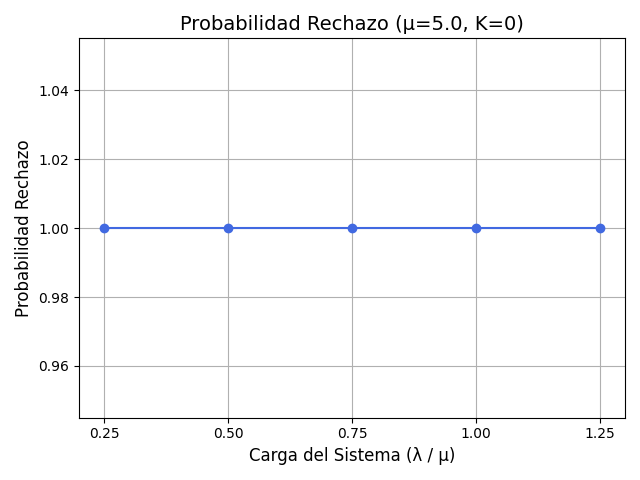
\includegraphics[width=0.48\textwidth]{graficas/mm1k/k_0/probabilidad_rechazo.png}
    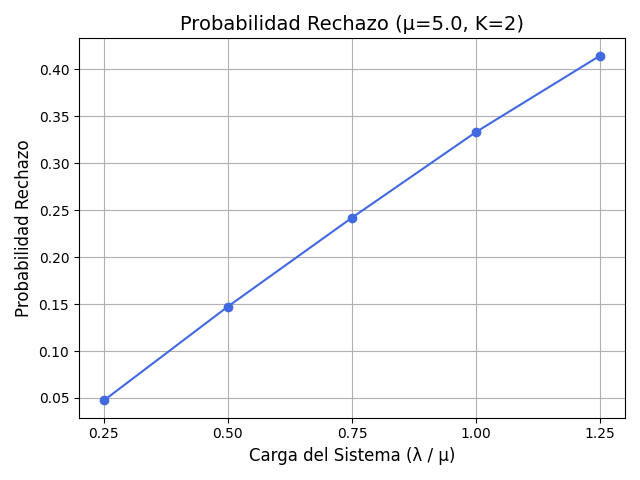
\includegraphics[width=0.48\textwidth]{graficas/mm1k/k_2/probabilidad_rechazo.png}
    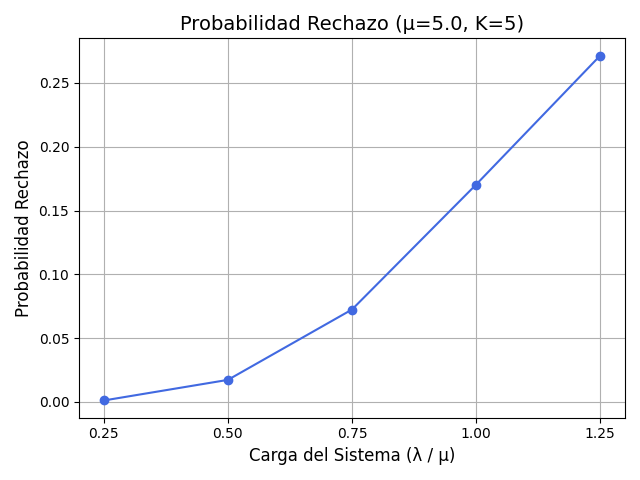
\includegraphics[width=0.48\textwidth]{graficas/mm1k/k_5/probabilidad_rechazo.png}
    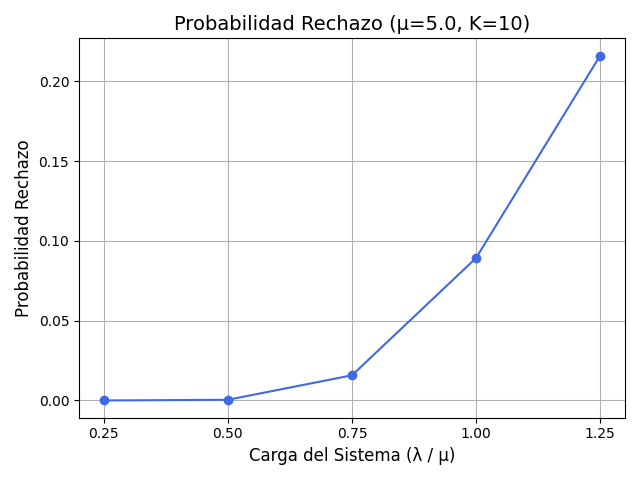
\includegraphics[width=0.48\textwidth]{graficas/mm1k/k_10/probabilidad_rechazo.png}
    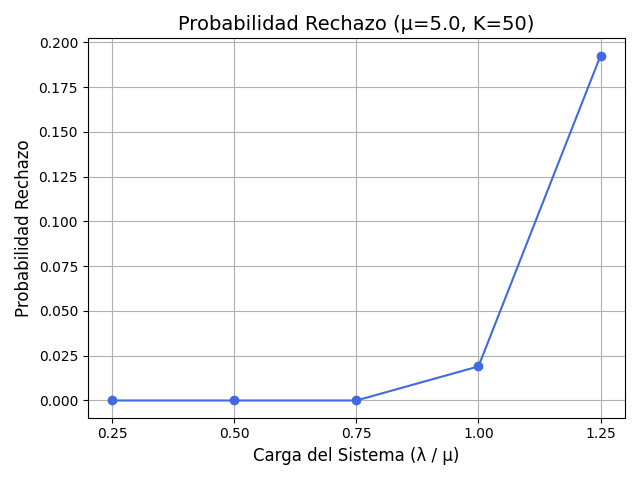
\includegraphics[width=0.48\textwidth]{graficas/mm1k/k_50/probabilidad_rechazo.png}
    \caption{Probabilidad de rechazo simulada para distintos valores de \( K \)}
\end{figure}

\textbf{Graficas de promedio en cola: }:
\begin{figure}[H]
    \centering
    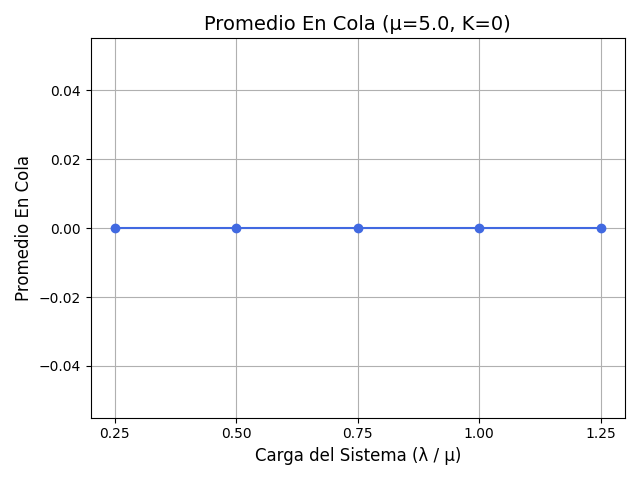
\includegraphics[width=0.48\textwidth]{graficas/mm1k/k_0/promedio_en_cola.png}
    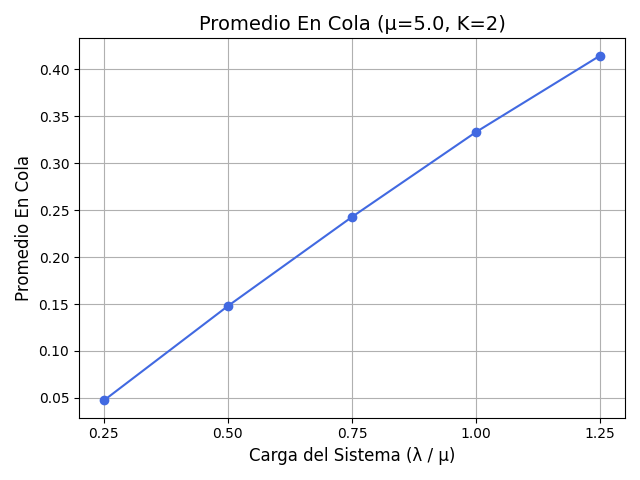
\includegraphics[width=0.48\textwidth]{graficas/mm1k/k_2/promedio_en_cola.png}
    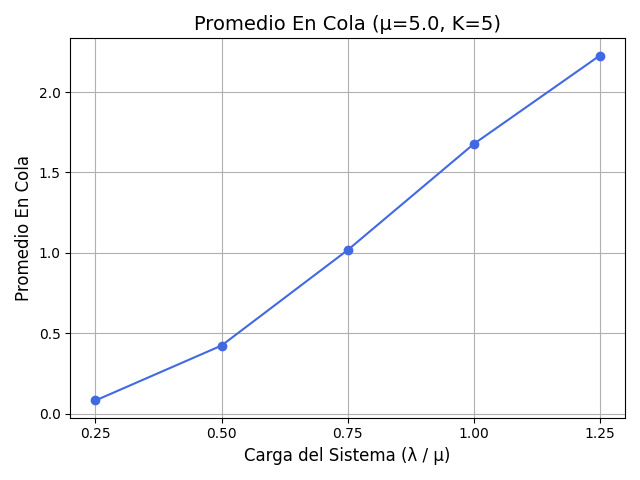
\includegraphics[width=0.48\textwidth]{graficas/mm1k/k_5/promedio_en_cola.png}
    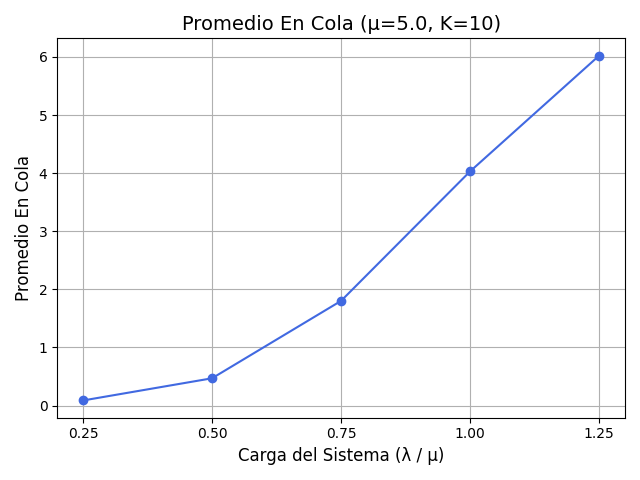
\includegraphics[width=0.48\textwidth]{graficas/mm1k/k_10/promedio_en_cola.png}
    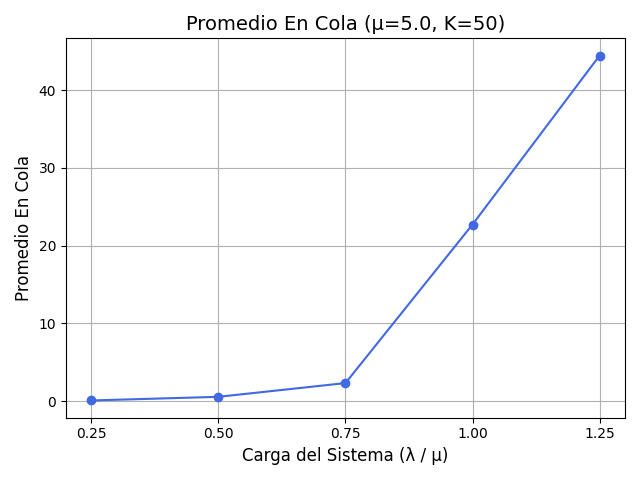
\includegraphics[width=0.48\textwidth]{graficas/mm1k/k_50/promedio_en_cola.png}
    \caption{Promedio de clientes en cola simulado para distintos valores de \( K \)}
\end{figure}


\textbf{Graficas de promedio en sistema: }:
\begin{figure}[H]
    \centering
    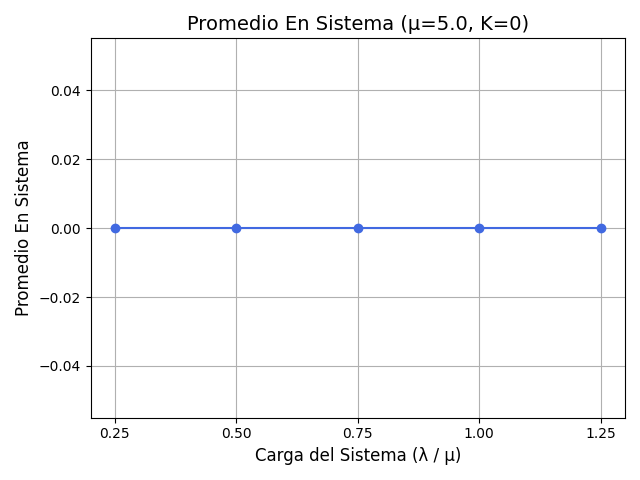
\includegraphics[width=0.48\textwidth]{graficas/mm1k/k_0/promedio_en_sistema.png}
    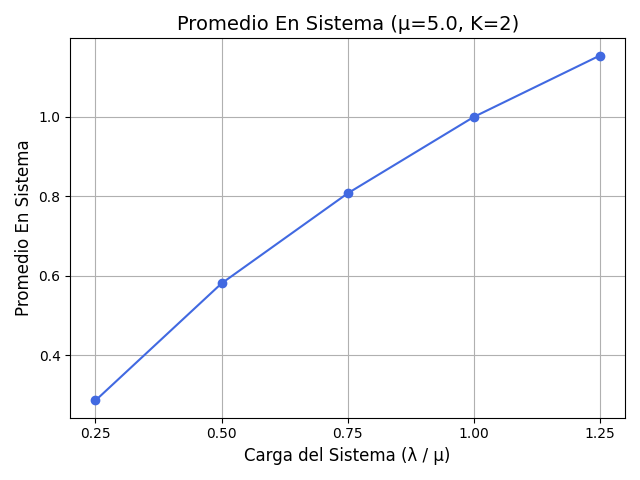
\includegraphics[width=0.48\textwidth]{graficas/mm1k/k_2/promedio_en_sistema.png}
    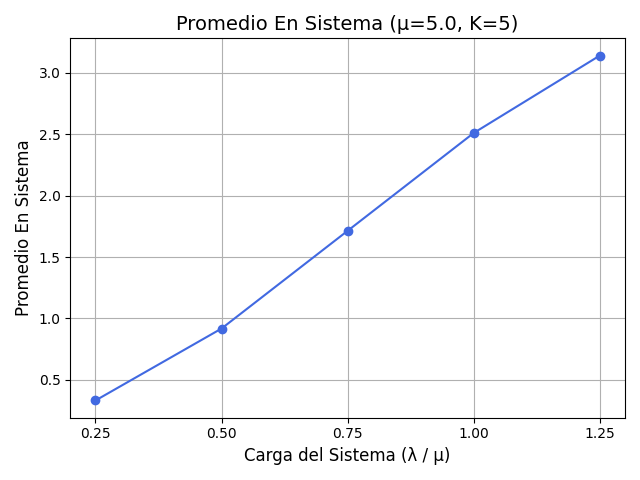
\includegraphics[width=0.48\textwidth]{graficas/mm1k/k_5/promedio_en_sistema.png}
    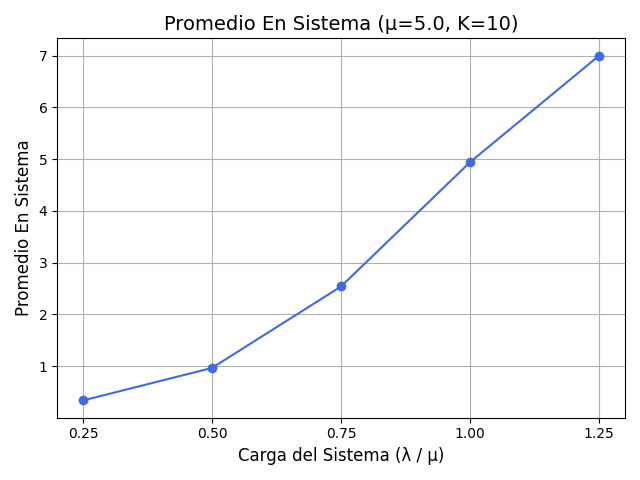
\includegraphics[width=0.48\textwidth]{graficas/mm1k/k_10/promedio_en_sistema.png}
    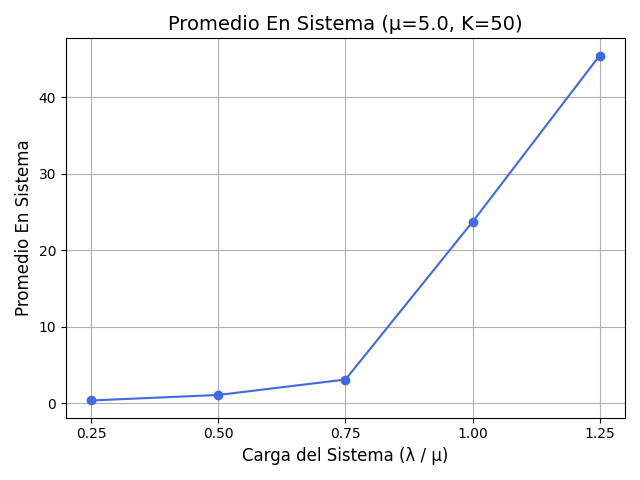
\includegraphics[width=0.48\textwidth]{graficas/mm1k/k_50/promedio_en_sistema.png}
    \caption{Promedio de clientes en el sistema simulado para distintos valores de \( K \)}
\end{figure}

\textbf{Graficas de tiempo promedio en cola: }:
\begin{figure}[H]
    \centering
    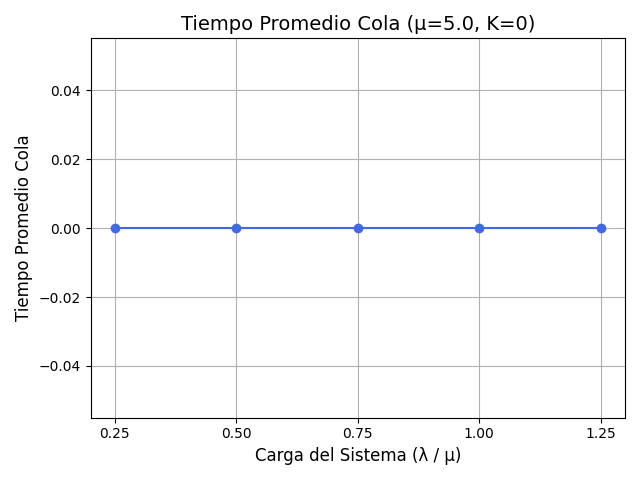
\includegraphics[width=0.48\textwidth]{graficas/mm1k/k_0/tiempo_promedio_cola.png}
    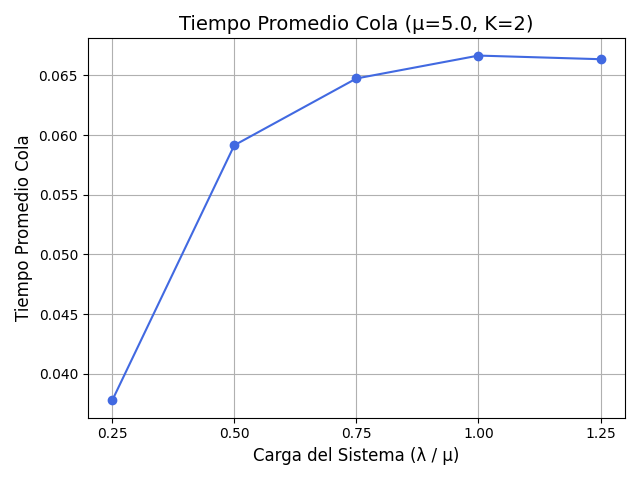
\includegraphics[width=0.48\textwidth]{graficas/mm1k/k_2/tiempo_promedio_cola.png}
    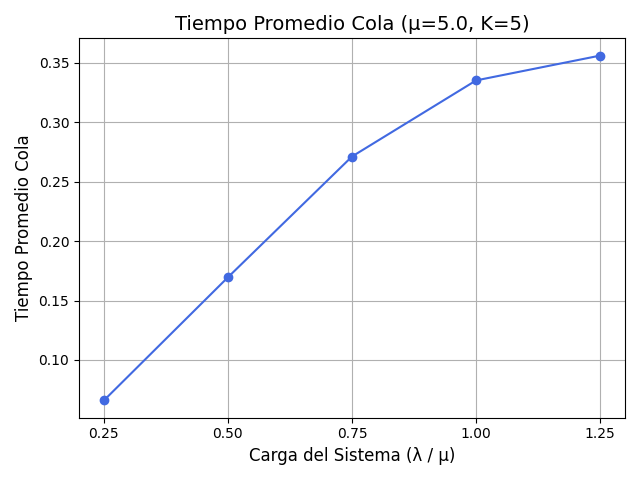
\includegraphics[width=0.48\textwidth]{graficas/mm1k/k_5/tiempo_promedio_cola.png}
    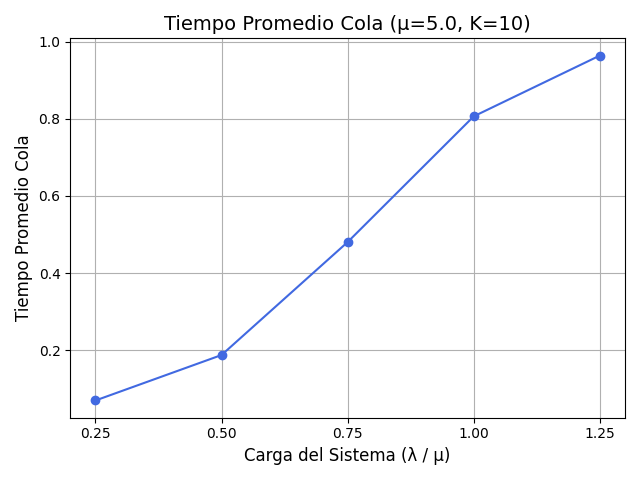
\includegraphics[width=0.48\textwidth]{graficas/mm1k/k_10/tiempo_promedio_cola.png}
    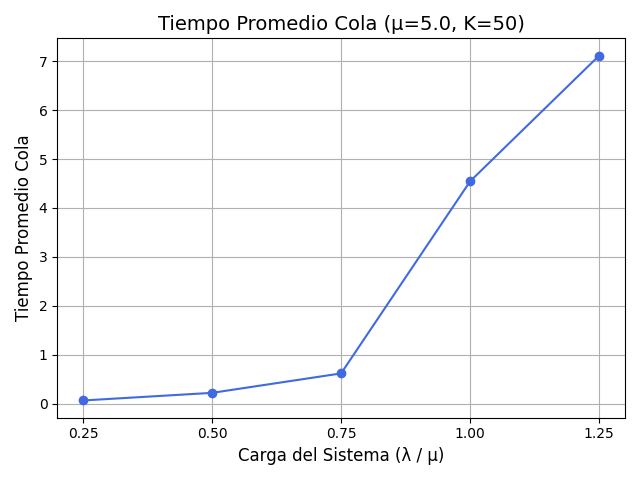
\includegraphics[width=0.48\textwidth]{graficas/mm1k/k_50/tiempo_promedio_cola.png}
    \caption{Promedio de tiempo en cola simulado para distintos valores de \( K \)}
\end{figure}


\textbf{Graficas de tiempo promedio en sistema: }:
\begin{figure}[H]
    \centering

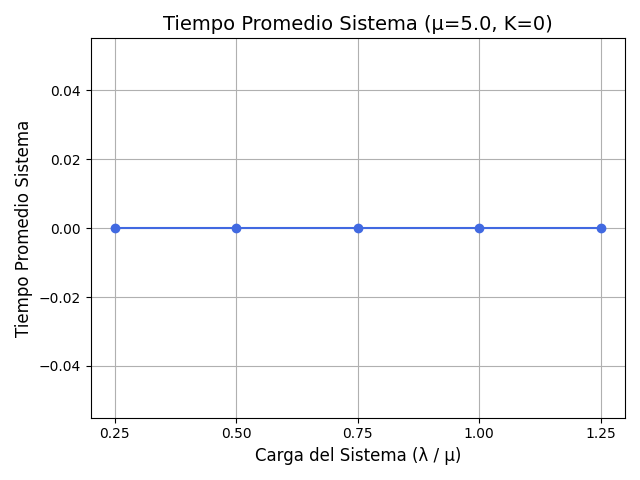
\includegraphics[width=0.48\textwidth]{graficas/mm1k/k_0/tiempo_promedio_sistema.png}
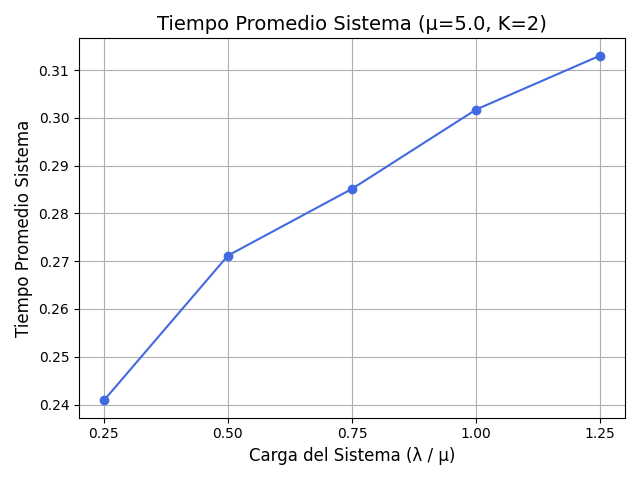
\includegraphics[width=0.48\textwidth]{graficas/mm1k/k_2/tiempo_promedio_sistema.png}
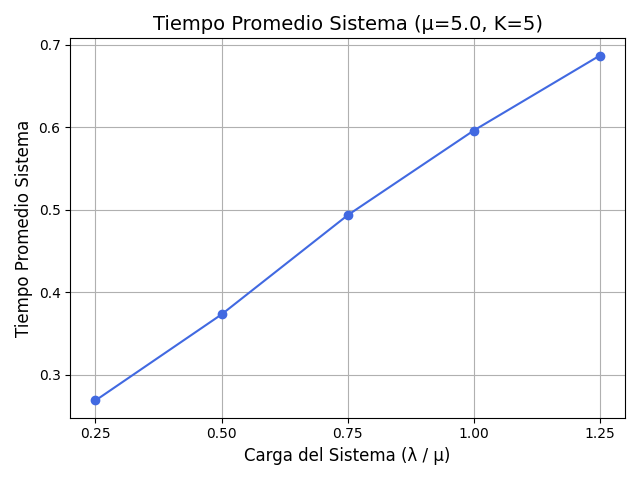
\includegraphics[width=0.48\textwidth]{graficas/mm1k/k_5/tiempo_promedio_sistema.png}
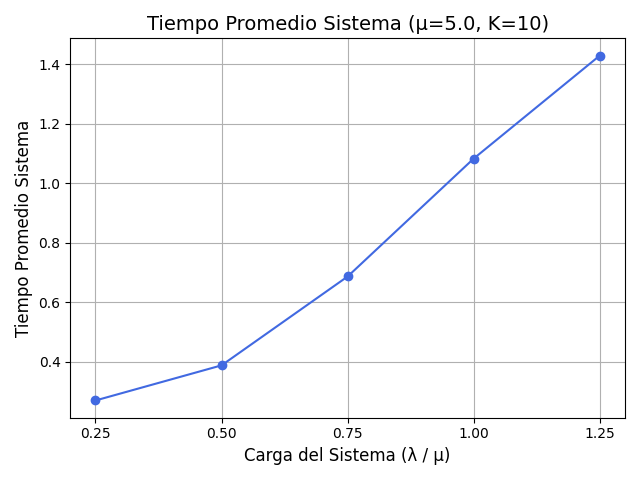
\includegraphics[width=0.48\textwidth]{graficas/mm1k/k_10/tiempo_promedio_sistema.png}
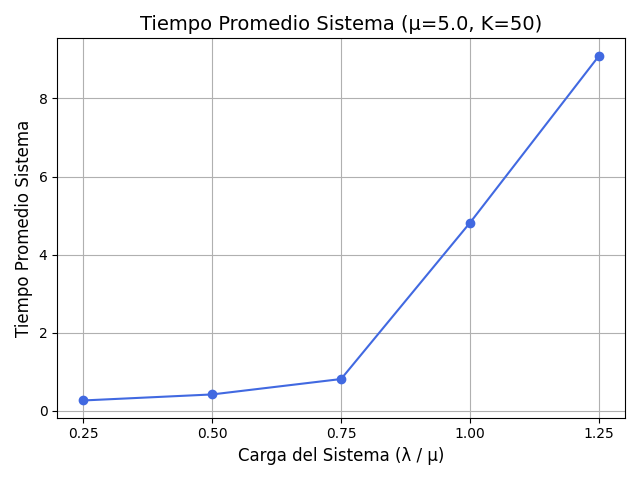
\includegraphics[width=0.48\textwidth]{graficas/mm1k/k_50/tiempo_promedio_sistema.png}
\caption{Promedio de tiempo en sistema simulado para distintos valores de \( K \)}
\end{figure}

\textbf{Graficas de utilizacion sistema: }:
\begin{figure}[H]
    \centering

    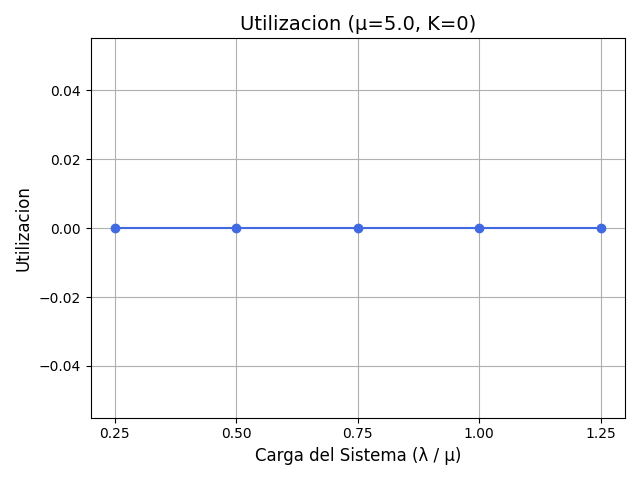
\includegraphics[width=0.48\textwidth]{graficas/mm1k/k_0/utilizacion.png}
    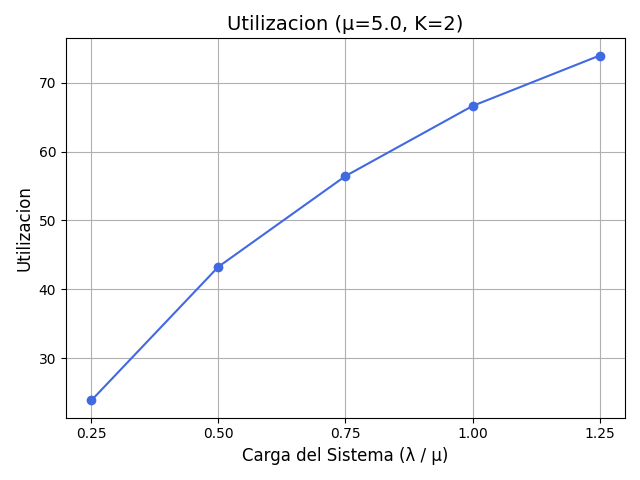
\includegraphics[width=0.48\textwidth]{graficas/mm1k/k_2/utilizacion.png}
    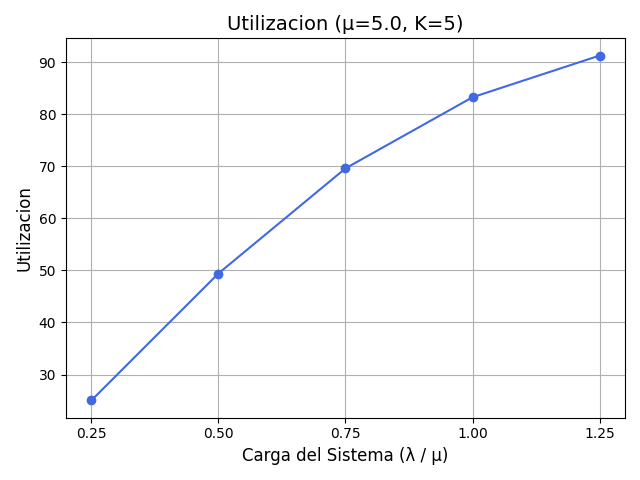
\includegraphics[width=0.48\textwidth]{graficas/mm1k/k_5/utilizacion.png}
    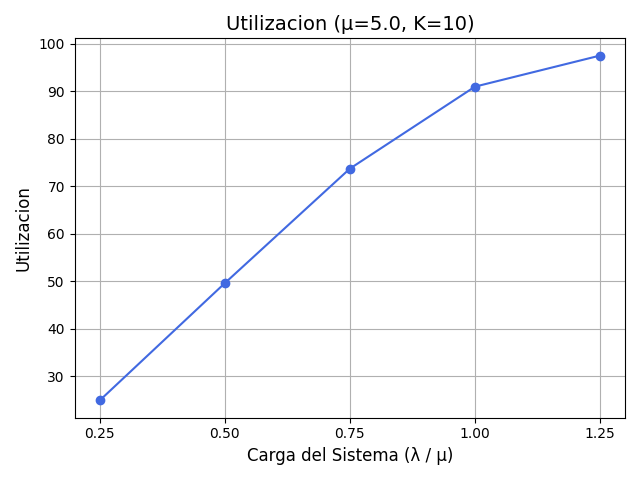
\includegraphics[width=0.48\textwidth]{graficas/mm1k/k_10/utilizacion.png}
    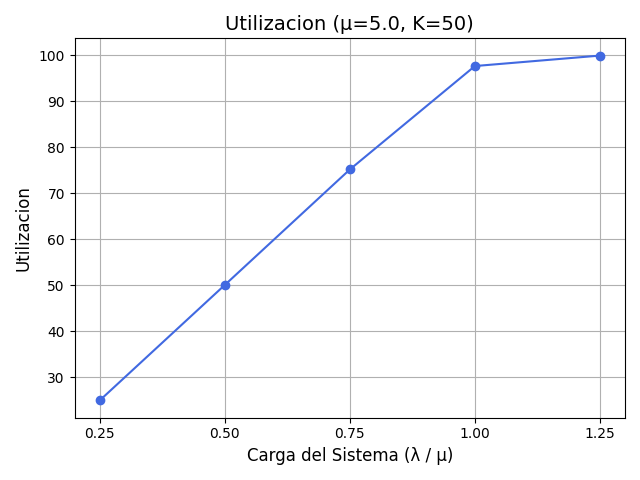
\includegraphics[width=0.48\textwidth]{graficas/mm1k/k_50/utilizacion.png}
    \caption{Utilizacion del sistema simulado para distintos valores de \( K \)}
\end{figure}

\subsubsection*{(b) Resultados Teóricos}

Los valores teóricos de la probabilidad de rechazo para el modelo M/M/1/K se calcularon utilizando la fórmula:

\[
P_K = \frac{(1 - \rho) \rho^K}{1 - \rho^{K+1}}, \quad \text{para } \rho \neq 1
\]

Los resultados obtenidos se resumen en la siguiente tabla:

\begin{table}[H]
\centering
\begin{tabular}{|c|c|c|c|c|c|}
\hline
\( \rho \) & \( K=0 \) & \( K=2 \) & \( K=5 \) & \( K=10 \) & \( K=50 \) \\
\hline
0.25 & 0 & 0.5 & 1.25 & 2.5 & 12.5 \\
0.50 & 0 & 1 & 2.5 & 5 & 25 \\
0.75 & 0 & 1.5 & 3.75 & 7.5 & 37.5 \\
1.00 & 0 & 2 & 5 & 10 & 50 \\
1.25 & 0 & 2.5 & 6.25 & 12.5 & 62.5 \\
\hline
\end{tabular}
\caption{Probabilidad teórica de rechazo \( P_K \) para distintos valores de \( \rho \) y \( K \)}
\end{table}

\subsubsection*{(c) Resultados en AnyLogic}

Se implementó un modelo equivalente en \textbf{AnyLogic} utilizando bloques estándar del entorno (Source, Queue, Server, Sink), parametrizados para replicar los valores de \( \lambda \), \( \mu \) y \( K \).

Para la comparación, se eligió una carga representativa del sistema: \( \rho = \lambda / \mu = 0.75 \), con \( \lambda = 3.75 \), \( \mu = 5 \).

A continuación se muestran los gráficos obtenidos para distintos valores de \( K \):

\begin{figure}[H]
    \centering
    \fbox{\parbox{0.7\textwidth}{
        \textbf{Nota:} No se presenta el gráfico para \( K = 0 \), ya que el modelo en AnyLogic no genera datos útiles bajo esta condición. Al no existir capacidad de cola ni disponibilidad inicial del servidor, el sistema no procesa clientes durante la simulación.
    }}
    \caption{Simulación no ejecutada para \( K = 0 \)}
\end{figure}


\begin{figure}[H]
    \centering
    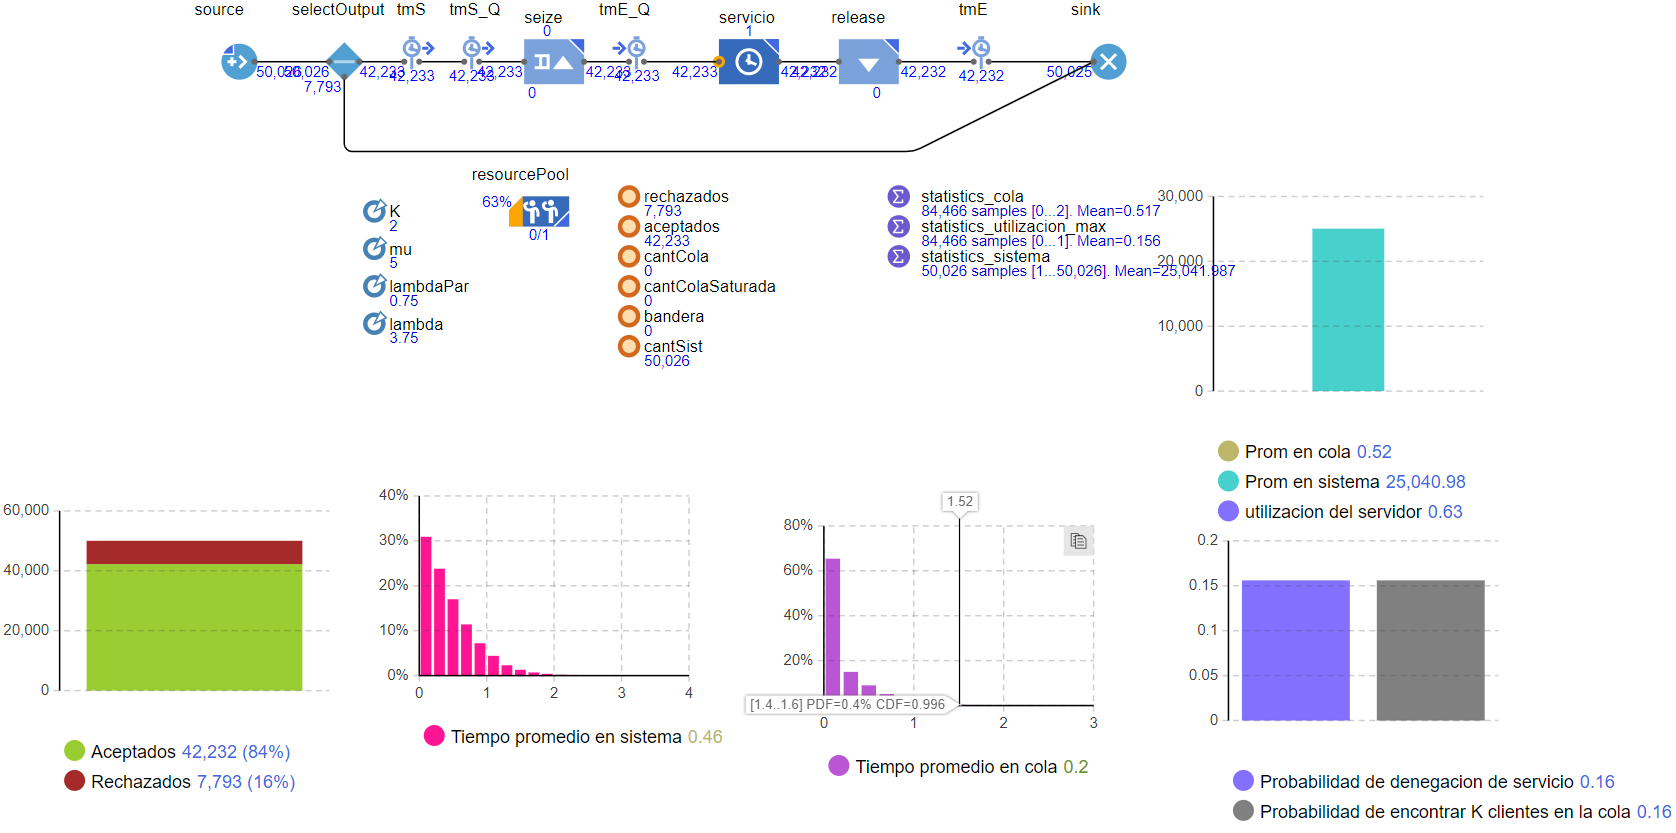
\includegraphics[width=0.75\textwidth]{./graficas/mm1k/anylogic/k_2.png}
    \caption{Resultados de AnyLogic para \( K = 2 \), con \( \lambda = 3.75 \)}
\end{figure}

\begin{figure}[H]
    \centering
    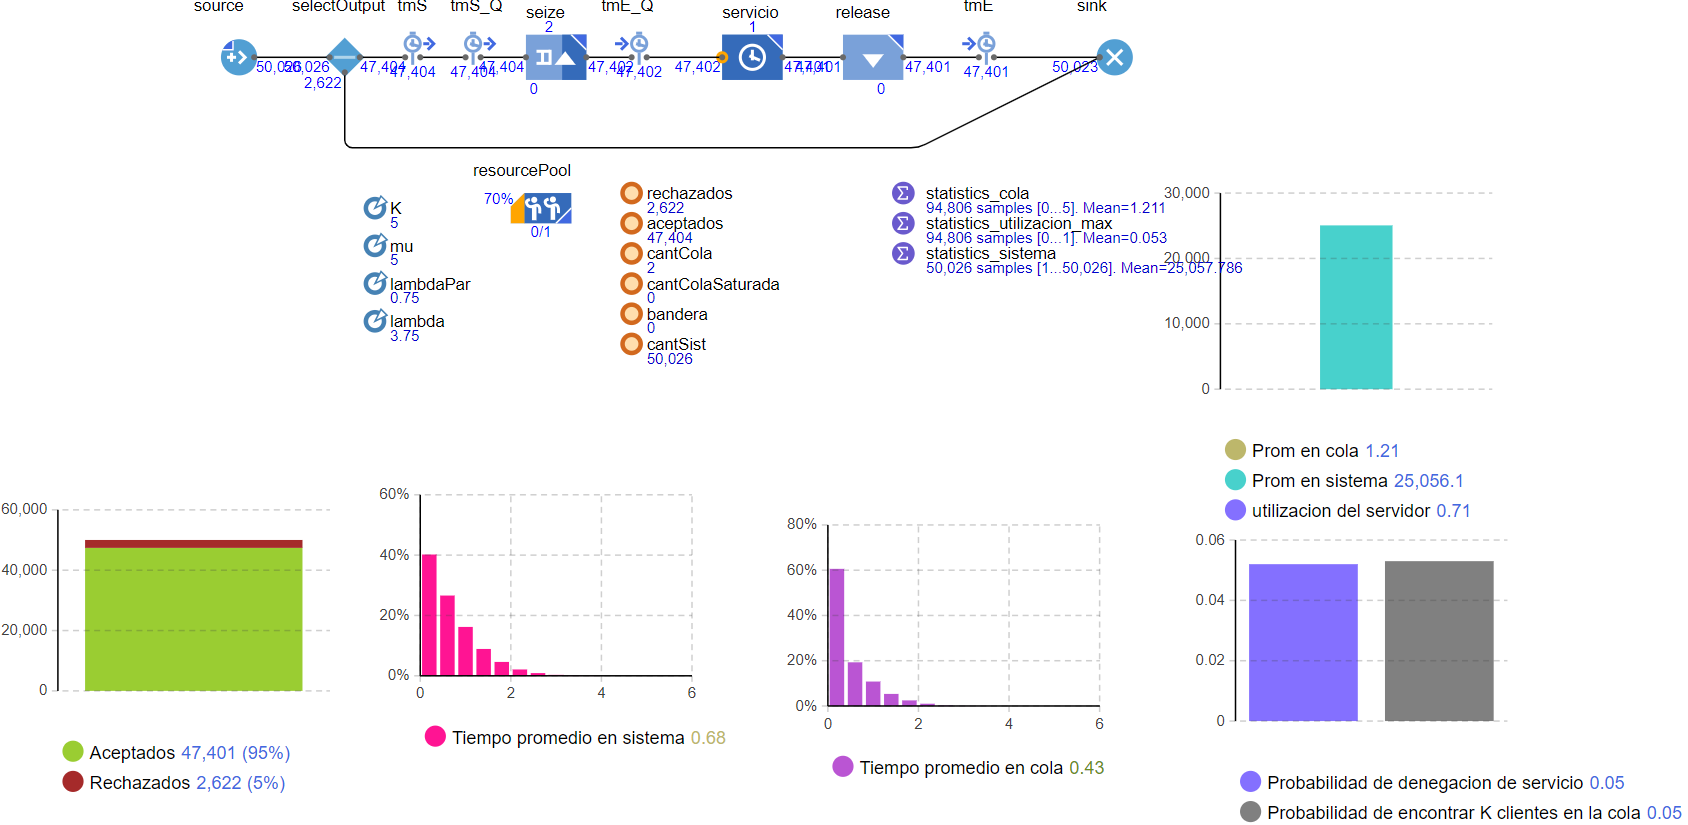
\includegraphics[width=0.75\textwidth]{./graficas/mm1k/anylogic/k_5.png}
    \caption{Resultados de AnyLogic para \( K = 5 \), con \( \lambda = 3.75 \)}
\end{figure}

\begin{figure}[H]
    \centering
    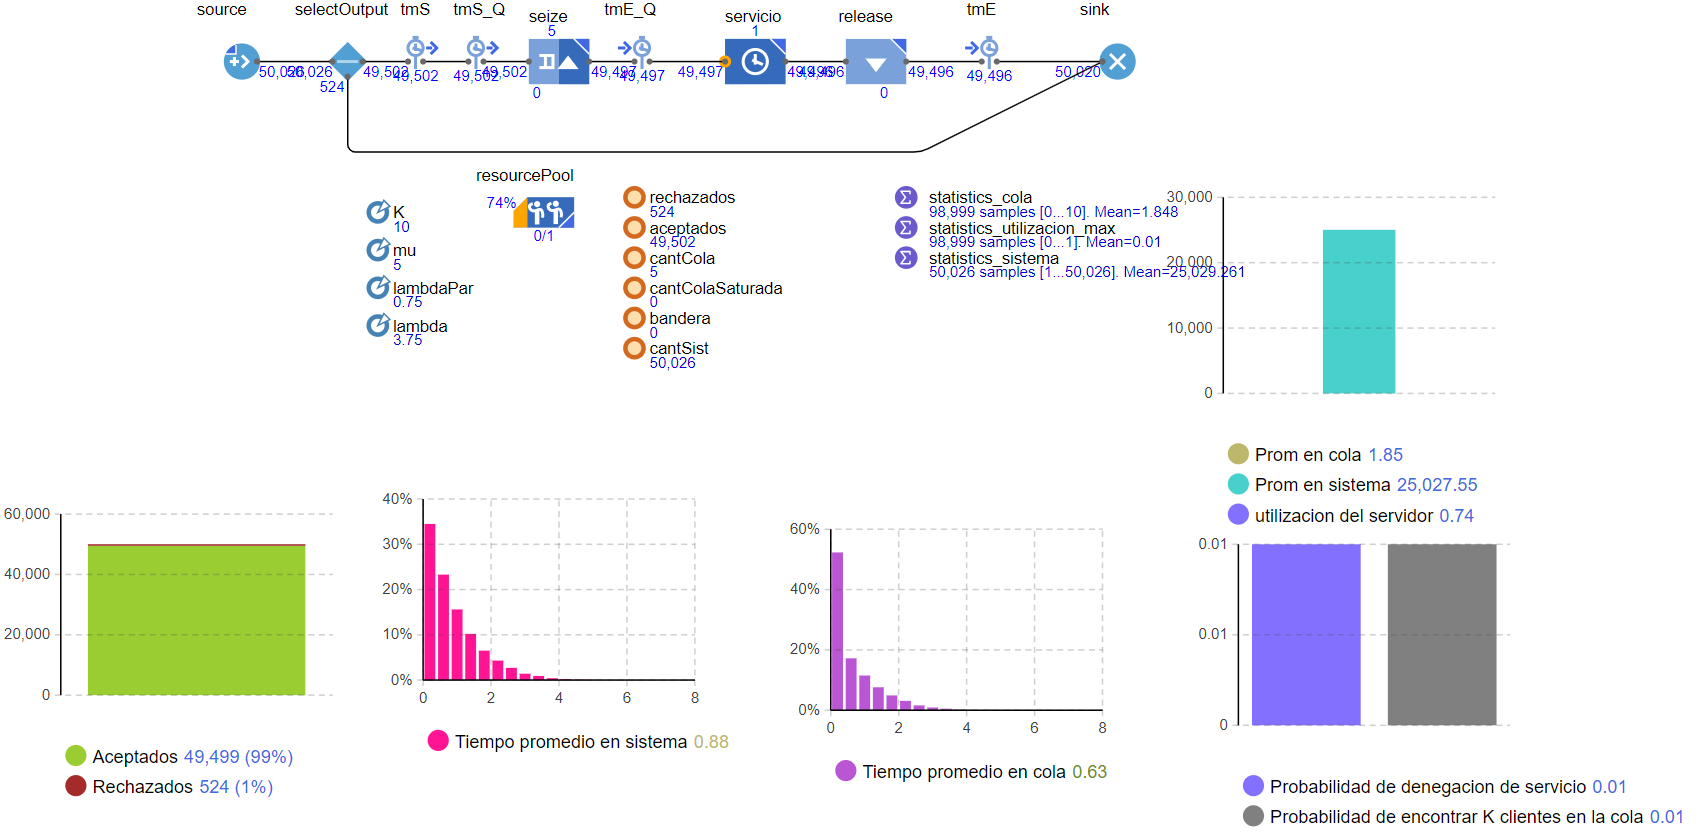
\includegraphics[width=0.75\textwidth]{./graficas/mm1k/anylogic/k_10.png}
    \caption{Resultados de AnyLogic para \( K = 10 \), con \( \lambda = 3.75 \)}
\end{figure}

\begin{figure}[H]
    \centering
    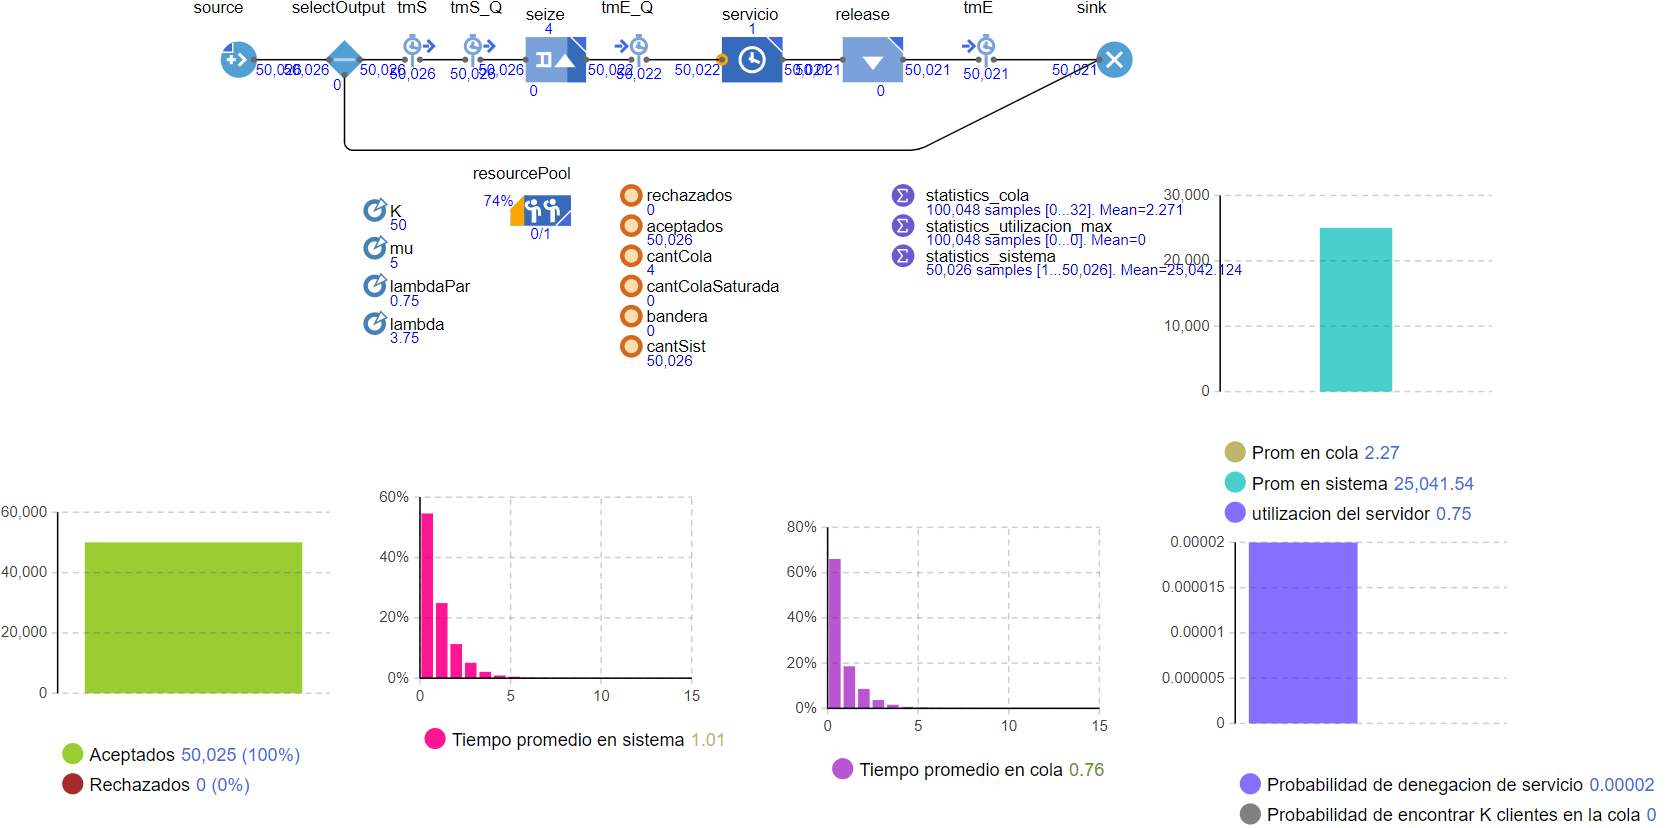
\includegraphics[width=0.75\textwidth]{./graficas/mm1k/anylogic/k_50.png}
    \caption{Resultados de AnyLogic para \( K = 50 \), con \( \lambda = 3.75 \)}
\end{figure}



\subsubsection*{(d) Comparación General}

Los tres enfoques (simulación en Python, resultados teóricos y simulación en AnyLogic) permiten observar una fuerte concordancia en la evolución de la probabilidad de rechazo respecto de la carga del sistema y el tamaño de la cola.

Dicha comparación valida la correcta implementación del modelo y la fidelidad de la simulación frente al análisis analítico.





%-------------------------------------
\subsection{Conclusiones del Modelo M/M/1}
%-------------------------------------
\begin{itemize}
    \item \textbf{Conclusión general del modelo M/M/1/K}\par
    La simulación del modelo M/M/1/K permitió analizar con precisión el comportamiento de un sistema de colas con un único servidor y capacidad finita, considerando distintas tasas de arribo relativas a la capacidad de servicio (\(\lambda\)/ \(\mu\)) y diversos tamaños máximos de cola (K=0;2,5;10;50). A partir de las métricas obtenidas en múltiples corridas por escenario, se lograron observaciones clave sobre la eficiencia operativa del sistema, el nivel de saturación, y el impacto directo de los recursos disponibles (capacidad de cola) frente a distintas demandas.
    \item \textbf{Influencia de la tasa de arribo (\(\lambda\)) sobre el desempeño del sistema}\par
    Uno de los hallazgos más notables es cómo la relación entre la tasa de arribo (\(\lambda\)) y la tasa de servicio (\(\mu\)) afecta todas las métricas de rendimiento. Al variar en porcentajes crecientes (25\%, 50\%, 75\%, 100\% y 125\% respecto de \(\mu\)), se observó:
    A bajas cargas (\(\lambda\)< \(\mu\)), el sistema permanece estable: las colas son mínimas, los tiempos de espera y en el sistema son bajos, y el servidor trabaja con baja ocupación. En estas condiciones, incluso una cola de tamaño 0 o 2 es suficiente para evitar rechazos de clientes, lo que permite ahorrar recursos sin comprometer el servicio.
    A medida que \(\lambda\) se acerca a \(\mu\) (cargas del 75\% al 100\%), el sistema entra en una zona crítica: se incrementan fuertemente los tiempos promedio en cola y en el sistema, el servidor tiende a estar ocupado casi permanentemente (alta utilización), y comienzan a aparecer rechazos frecuentes si el tamaño de la cola es limitado
    Para valores de \(\lambda\)> \(\mu\) (125 \% de carga), se confirma la saturación del sistema: el servidor no puede atender a todos los clientes que llegan, y la probabilidad de denegación de servicio se dispara, especialmente en colas pequeñas. En este régimen, el sistema es inestable si la capacidad no es suficiente, generando altos niveles de pérdida de clientes y colas crecientes (si fueran infinitas).
    \item \textbf{Impacto del tamaño de la cola (K) en el rendimiento}\par
    El segundo eje de análisis fue la variación del parámetro K, que representa la capacidad máxima del sistema (servidor + cola). Comparando los resultados entre colas de tamaño 0, 2, 5, 10 y 50, se identificaron los siguientes patrones:
    Una cola de tamaño 0 (K=1) implica que si el servidor está ocupado, cualquier cliente que llegue será rechazado. Esto genera una altísima probabilidad de denegación de servicio, incluso con cargas moderadas (por ejemplo, \(\lambda\)=0.75\(\mu\)).

    Al aumentar ligeramente la cola a K=2 o K=5, el sistema mejora considerablemente: el número de rechazos disminuye y se absorbe mejor la variabilidad en los tiempos de llegada. Sin embargo, bajo cargas cercanas o superiores a  \(\mu\), estas colas pequeñas aún resultan insuficientes, con una probabilidad de rechazo significativa y tiempos en cola elevados.

    En el caso de colas más amplias (K=10 y K=50), el sistema puede soportar cargas más altas sin rechazar tantos clientes. A medida que crece K, la probabilidad de denegación disminuye drásticamente, lo cual se traduce en una mejora del nivel de servicio, aunque con un costo mayor asociado al espacio de espera y al tiempo que los clientes deben permanecer en cola.
    \item \textbf{Análisis conjunto: tasa de arribo vs.tamaño de la cola}\par
    El análisis cruzado de ambas variables revela una interacción crítica entre la demanda y la capacidad del sistema:

    A bajas tasas de arribo, el tamaño de la cola tiene un efecto marginal: incluso valores bajos de K bastan para mantener un buen desempeño.

    A tasas de arribo altas, el sistema necesita colas más largas para evitar rechazos, pero esto conlleva un aumento en el tiempo de espera.

    Existe un punto de equilibrio entre tamaño de cola y nivel de carga, donde el sistema logra un buen trade-off entre utilización del servidor, nivel de servicio, y minimización del tiempo en sistema.

    Se concluye que para lograr eficiencia y calidad de servicio, es indispensable dimensionar la cola en función de la tasa de arribo esperada. Aumentar la capacidad de espera no siempre soluciona el problema: si \(\lambda\)>\(\mu\), la congestión es inevitable sin cambiar la tasa de servicio (es decir, sin agregar más servidores o mejorar el procesamiento).
    \item \textbf{Qué tan bien se aproximan las simulaciones a la teoría.}\par
    En el modelo teórico de colas M/M/1 (es decir, sin límite de capacidad), existen fórmulas bien definidas para calcular medidas como:
    \begin{itemize}
        \item Utilización del servidor ($\rho = \frac{\lambda}{\mu}$).
        \item Promedio de clientes en el sistema ($L = \frac{\lambda}{\mu - \lambda}$).
        \item Promedio de clientes en la cola ($L_q = \frac{\lambda^2}{\mu(\mu - \lambda)}$).
        \item Tiempo promedio en el sistema ($W = \frac{1}{\mu - \lambda}$).
        \item Tiempo promedio en la cola ($W_q = \frac{\lambda}{\mu(\mu - \lambda)}$).
    \end{itemize}

    Pero estas fórmulas solo son válidas cuando la tasa de llegada \(\lambda\) es menor que la tasa de servicio \(\mu\).

    Cuando lambda es mayor o igual a mu:

    El sistema entra en una situación inestable.

    El número de clientes en cola crece indefinidamente.

    Los tiempos de espera se vuelven infinitos.

    No se puede aplicar la teoría porque no se llega a un estado estable.
    La ventaja de la simulación es que sí podemos ejecutar el sistema aunque lambda sea igual o mayor que mu, y observar qué pasa en un período de tiempo finito (por ejemplo, 1000 minutos).

    Particularmente en el modelo M/M/1/K (con cola finita), incluso si la llegada de clientes supera la capacidad de atención, la simulación no se rompe: simplemente empieza a rechazar clientes cuando ya no hay espacio disponible.

    Esto permite ver cómo:
    \begin{itemize}
        \item La utilización del servidor se acerca al 100\% cuando lambda es alta.
        \item Los tiempos de espera aumentan significativamente.
        \item La cantidad de clientes rechazados crece a medida que la tasa de llegada supera la capacidad del sistema.
        \item El sistema se mantiene artificialmente estable solo porque tiene un límite en la cantidad de clientes que puede albergar (el tamaño K de la cola).
    \end{itemize}
    Como conclusion, notamos que la teoría proporciona resultados analíticos valiosos, pero queda limitada a escenarios donde el sistema está en equilibrio. Cuando la demanda es mayor que la capacidad (lambda mayor o igual que mu), solo la simulación permite estudiar el comportamiento del sistema de forma realista, mostrando fenómenos como saturación, congestión y pérdida de clientes.

    Este contraste evidencia el valor de la simulación como herramienta complementaria a la teoría, ya que permite observar dinámicas complejas que en la teoría no pueden modelarse, especialmente en sistemas con capacidad finita o condiciones extremas de carga.
    \item Diferencias observadas entre Python y AnyLogic.
    \item \textbf{Probabilidad de rechazo en colas finitas.}\par
    La probabilidad de rechazo aparece en los modelos con cola limitada, como el modelo M/M/1/K. Representa la fracción de clientes que intentan ingresar al sistema, pero no pueden hacerlo porque tanto el servidor como la cola se encuentran ocupados al momento de su llegada.

    En términos prácticos, un cliente rechazado es un cliente perdido: no ingresa al sistema, no espera,su atención no es procesada y el cliente no vuelve tampoco. Esta métrica es clave en escenarios donde el objetivo es minimizar pérdidas de atención, tiempos de espera, o maximizar la eficiencia del sistema.

    A partir de los resultados obtenidos en la simulación, variando tanto la tasa de arribo como la capacidad del sistema (valor de $K$), se observaron los siguientes patrones:

    \begin{itemize}
        \item \textbf{A menor tamaño de cola ($K$), mayor probabilidad de rechazo.} En sistemas con $K = 0$ (es decir, sin espacio para esperar), cualquier cliente que llega y encuentra al servidor ocupado es inmediatamente rechazado. Esto genera una probabilidad de rechazo elevada incluso con tasas de llegada moderadas.
        
        \item \textbf{La probabilidad de rechazo disminuye al aumentar $K$.} A medida que se incrementa la capacidad de espera, el sistema puede contener a más clientes simultáneamente, lo que reduce las pérdidas. Esta reducción es especialmente notoria en escenarios donde la tasa de arribo se aproxima a la tasa de servicio.
        
        \item \textbf{Con cargas bajas (por ejemplo, cuando $\lambda < 0{,}5 \mu$), la probabilidad de rechazo es prácticamente nula, incluso con valores bajos de $K$.} En estos casos, los clientes rara vez encuentran el sistema saturado.
        
        \item \textbf{Con cargas altas ($\lambda \geq \mu$), incluso con colas amplias, la probabilidad de rechazo sigue siendo significativa.} Aunque un mayor valor de $K$ reduce el rechazo, este nunca desaparece por completo cuando la tasa de llegada supera la capacidad de atención del servidor.
    \end{itemize}

    Desde el punto de vista teórico, la probabilidad de rechazo en un sistema M/M/1/K se puede calcular mediante una fórmula cerrada que depende del valor de $K$ y de la relación $\rho = \lambda / \mu$. Esta fórmula muestra que, cuando la carga es alta, el rechazo crece rápidamente si la cola no es lo suficientemente grande.

    La simulación confirmó estos comportamientos y permitió visualizar cómo la probabilidad de rechazo se comporta bajo diferentes configuraciones del sistema. Además, demostró que es posible modelar situaciones de saturación sin depender exclusivamente de la estabilidad teórica, obteniendo estimaciones precisas de pérdidas y rendimiento aún en escenarios no estacionarios.

    En conclusión, la probabilidad de rechazo es un indicador crucial para el diseño de sistemas eficientes. Dimensionar adecuadamente el tamaño de la cola no solo minimiza pérdidas, sino que permite alcanzar niveles aceptables de calidad de servicio sin sobredimensionar recursos. La simulación, en este contexto, se presenta como una herramienta poderosa para anticipar comportamientos y tomar decisiones estratégicas fundamentadas.
    \item \textbf{Conclusión final del modelo M/M/1/K}\par
    El modelo M/M/1/K, a pesar de su simplicidad matemática, permite representar con gran claridad problemas reales de capacidad limitada, como cajeros automáticos, estaciones de servicio, llamadas en centros de atención o turnos en clínicas. La simulación confirmó el marco teórico clásico, donde las colas finitas imponen una restricción severa al sistema cuando la demanda se aproxima o supera a la capacidad de atención, mientras que con la solucion analitica se pueden obtener métricas precisas para evaluar el rendimiento del sistema. Con la simulacion en anylogic se pudo observar el comportamiento del sistema en tiempo real, lo que permitió validar las métricas obtenidas y analizar la dinámica de la cola bajo diferentes condiciones de carga y capacidad.

    El análisis detallado de métricas como el tiempo promedio en cola, la utilización del servidor, y la probabilidad de rechazo, proporcionó criterios objetivos para la toma de decisiones sobre capacidad, planificación de recursos y diseño de infraestructura. En suma, el modelo M/M/1/K demostró ser una herramienta robusta y flexible para evaluar el rendimiento de sistemas reales bajo restricciones operativas concretas.


\end{itemize}

%===========================================================
\section{Modelo de Inventario (s, S)}
%===========================================================

\subsection{Marco Teórico}

El modelo de inventario $(s, S)$ es una política de revisión periódica en la que:

\begin{itemize}
    \item Se monitorea diariamente el inventario disponible.
    \item Si el nivel baja a $s$ o menos y no hay un pedido pendiente, se ordena la cantidad necesaria para alcanzar el nivel $S$.
    \item La demanda diaria sigue una distribución de Poisson con media \( \lambda \).
    \item El pedido llega luego de un \textit{lead time} constante \( l \).
\end{itemize}

No se considera acumulación de faltantes (backordering): la demanda no satisfecha se pierde y genera un costo inmediato.

\textbf{Costos involucrados:}
\begin{itemize}
    \item \textbf{Costo de orden} ($C_{\text{orden}}$): se incurre cada vez que se emite un pedido.
    \item \textbf{Costo de mantenimiento} ($C_{\text{mant}}$): proporcional a las unidades almacenadas por día.
    \item \textbf{Costo de faltante} ($C_{\text{falt}}$): proporcional a las unidades no satisfechas.
\end{itemize}

El costo total acumulado durante el horizonte de simulación se calcula como:

\[
C_{\text{total}} = \sum_{t=1}^{T} \left( C_{\text{orden}}(t) + C_{\text{mant}}(t) + C_{\text{falt}}(t) \right)
\]


\subsection{Implementación en Python}

Se desarrolló una simulación basada en pasos discretos diarios. En cada día:
\begin{itemize}
    \item Se simula la demanda con una distribución de Poisson.
    \item Se actualiza el nivel de inventario.
    \item Se contabilizan los costos correspondientes.
    \item Si se alcanza el punto de reorden $s$ y no hay un pedido pendiente, se ordena hasta $S$.
\end{itemize}

\textbf{Aspectos destacados:}
\begin{itemize}
    \item Control explícito del lead time: los pedidos llegan luego de $l$ días.
    \item Cálculo acumulativo de costos diarios de mantenimiento y faltantes.
    \item Repetición de múltiples corridas para calcular promedios estables.
\end{itemize}

\textbf{Métricas evaluadas:}
\begin{itemize}
    \item Costo total.
    \item Costo de orden.
    \item Costo de mantenimiento.
    \item Costo por faltantes.
\end{itemize}

\textbf{Ejemplo de ejecución desde consola:}
\begin{verbatim}
python3 sim-modelo-inventario.py --s 20 --S 80 --d 6 --t 365 --co 100 --cm 0.5 --cf 10 --l 2 --c 30
\end{verbatim}


%-------------------------------------
\subsection{Simulación en AnyLogic}
%-------------------------------------

Con el objetivo de validar los resultados obtenidos mediante la simulación en Python, se desarrolló una versión equivalente del modelo de inventario $(s, S)$ en la plataforma de simulación \textbf{AnyLogic}.

El modelo fue construido utilizando componentes estándar del entorno de simulación de eventos discretos, y refleja fielmente la dinámica del sistema bajo análisis, incorporando la demanda diaria, los pedidos con \textit{lead time}, y la evaluación de los niveles de inventario.

\subsubsection*{Estructura del modelo}

La estructura principal del modelo en AnyLogic incluye los siguientes bloques:

\begin{itemize}
    \item \texttt{Source}: genera una entidad por día, representando un paso del tiempo.
    \item \texttt{Delay} (bloque de tiempo): simula el proceso diario y permite ejecutar la lógica de simulación al ritmo de un día por entidad.
    \item \texttt{SelectOutput}: ramifica el flujo para aplicar la lógica de reorden.
    \item \texttt{Queue / Delay / Release}: representan el ciclo de entrega de los pedidos.
    \item Variables auxiliares: controlan el inventario, el pedido pendiente y los costos acumulados.
\end{itemize}

\vspace{0.5em}
\begin{figure}[H]
    \centering
    \includegraphics[width=0.9\textwidth]{graficas/modelos/ModeloMM1/diagrama_mm1.png}
    \caption{Estructura del modelo $(s, S)$ implementado en AnyLogic.}
\end{figure}

\subsubsection*{Justificación de parámetros utilizados}

Se definieron los siguientes valores de referencia para realizar la simulación:

\begin{itemize}
    \item Punto de reorden: \( s = 20 \)
    \item Nivel máximo: \( S = 80 \)
    \item Demanda diaria media: \( \lambda = 5 \)
    \item Lead time: \( l = 2 \) días
    \item Horizonte de simulación: \( T = 100\) días
\end{itemize}

Estos parámetros coinciden con los utilizados en la simulación en Python, permitiendo una comparación directa de resultados.

\subsubsection*{Eventos y variables clave}

El modelo incluye las siguientes variables y eventos personalizados:

\begin{itemize}
    \item \texttt{inventario} (int): representa el inventario disponible día a día.
    \item \texttt{pedidoPendiente} (boolean): indica si hay un pedido en curso.
    \item \texttt{diasParaEntrega} (int): cuenta regresiva para el arribo del pedido.
    \item \texttt{demandaDiaria}: generada con distribución de Poisson.
    \item \texttt{costosAcumulados}: incluye costos de orden, mantenimiento y faltantes.
\end{itemize}

La lógica de reorden se implementa dentro de un bloque de código ejecutado cada día, que evalúa si el inventario cayó por debajo del punto de reorden y, en ese caso, genera un pedido cuya llegada se programa a \( t + l \) días.

\subsubsection*{Graficos de resultados}

Durante la simulación se registran las métricas clave de interés:

\begin{itemize}
    \item Evolución del inventario.
    \item Costo total acumulado.
    \item Costos individuales (orden, mantenimiento, faltantes).
    \item Cantidad de pedidos emitidos.
\end{itemize}

\begin{figure}[H]
    \centering
    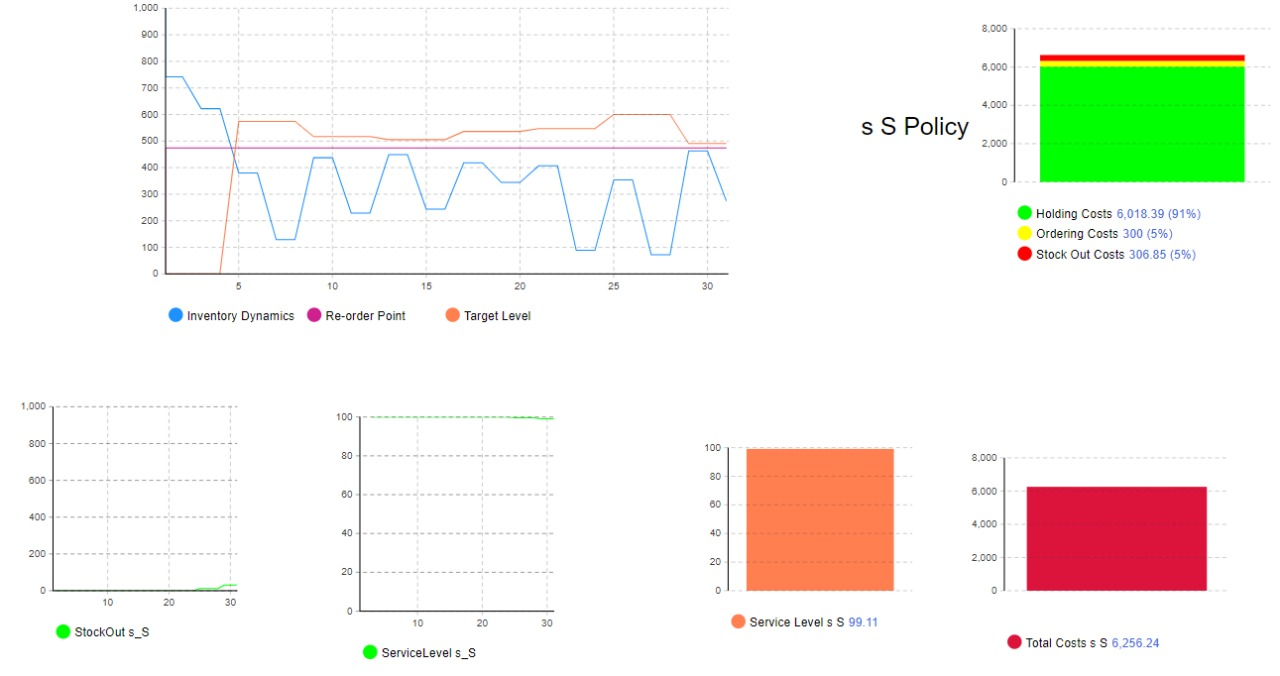
\includegraphics[width=0.9\textwidth]{./graficas/modelos/inventario/evolucion.jpg}
    \caption{Gráfico de evolución del inventario simulado en AnyLogic.}
\end{figure}

%-------------------------------------
\subsection{Resultados y Gráficas}
%-------------------------------------
\subsubsection*{Gráficas Generadas}

\begin{figure}[H]
    \centering
    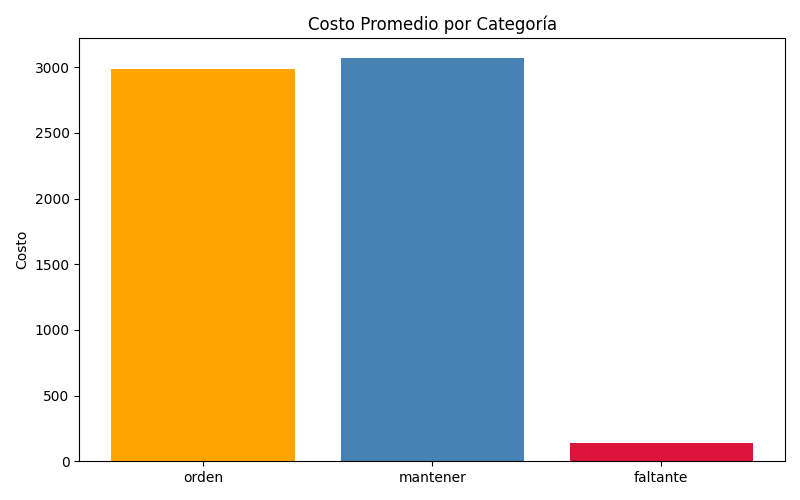
\includegraphics[width=0.48\textwidth]{graficas/costos/costos_promedio.png}
    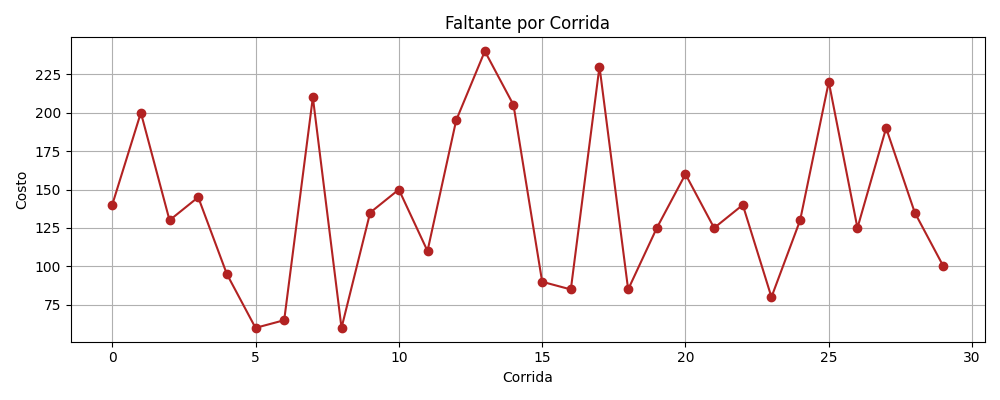
\includegraphics[width=0.48\textwidth]{graficas/costos/faltante_por_corrida.png}
    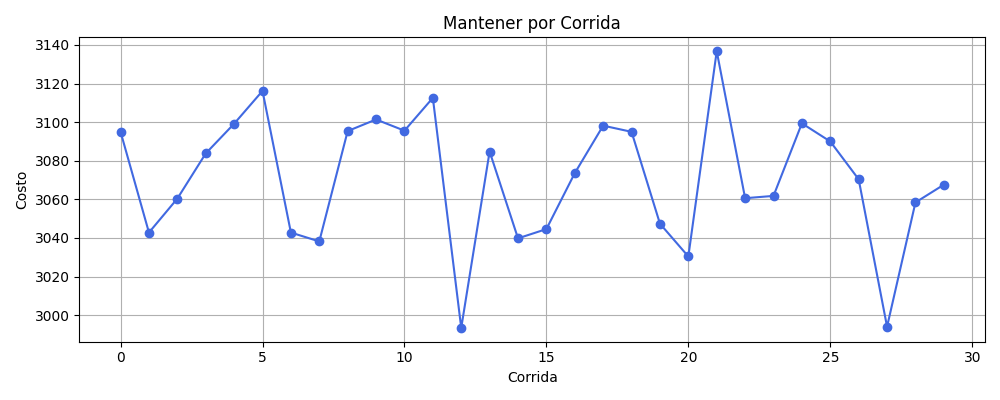
\includegraphics[width=0.48\textwidth]{graficas/costos/mantener_por_corrida.png}
    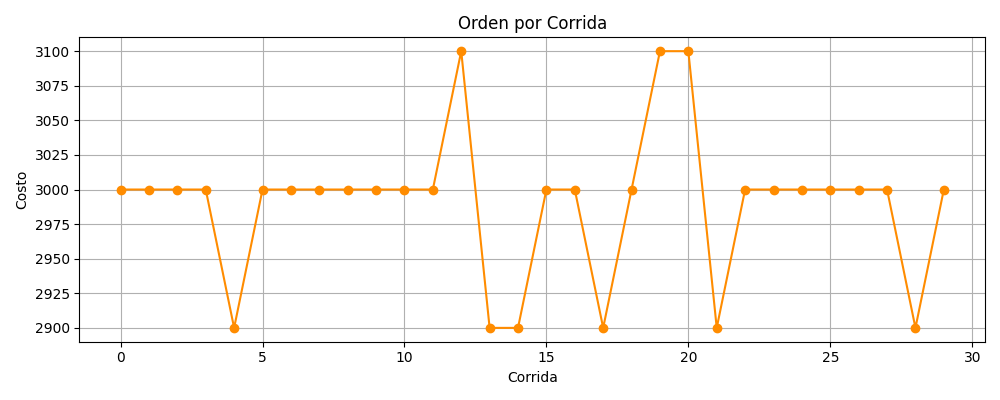
\includegraphics[width=0.48\textwidth]{graficas/costos/orden_por_corrida.png}
    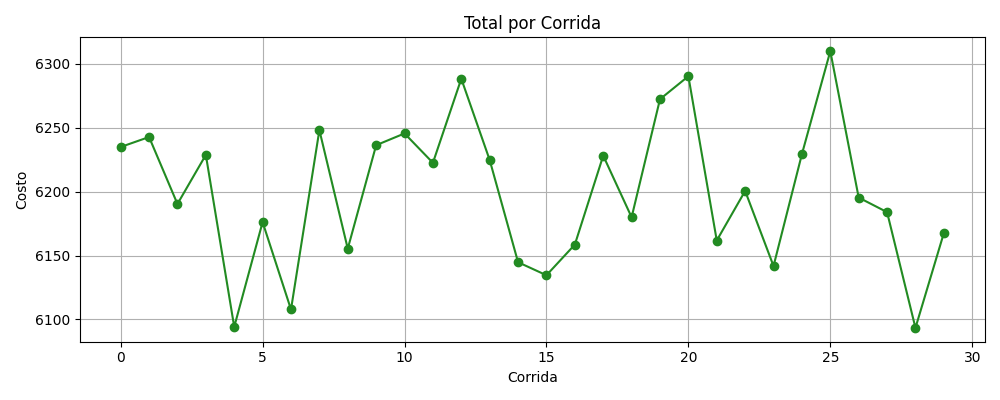
\includegraphics[width=0.48\textwidth]{graficas/costos/total_por_corrida.png}
    
    \caption{Costos del inventario simulados en python}
\end{figure}

\subsection{Conclusiones del Modelo de Inventario}
\begin{itemize}
    \item \textbf{Comportamiento del inventario frente a variaciones de demanda y lead time:}  
    El modelo de inventario basado en la política $(s, S)$ mostró un comportamiento dinámico ante la variabilidad de la demanda generada mediante una distribución de Poisson. Se observó que, a pesar de las fluctuaciones aleatorias en la demanda y en el tiempo de entrega (lead time), el sistema logró mantener el inventario dentro de márgenes operativos seguros. Los períodos en que el inventario descendía por debajo del punto de reorden eran compensados por pedidos emitidos oportunamente, reduciendo así el riesgo de desabastecimiento prolongado.

    \item \textbf{Relación entre costos y parámetros $(s, S)$:}  
    Los resultados evidenciaron que los costos de mantenimiento y orden fueron los componentes más significativos del costo total. En particular, el costo de mantenimiento representó el mayor porcentaje (más del 90\% en algunas simulaciones con AnyLogic), mientras que los costos por faltante se mantuvieron bajos gracias a la adecuada configuración de los parámetros $s = 20$ y $S = 80$. Estos valores permitieron alcanzar un nivel de servicio superior al 99\%, con un control eficiente del inventario y los costos asociados.

    \item \textbf{Coincidencias entre métodos:}  
    La comparación entre los resultados obtenidos en Python y los generados en AnyLogic reveló una alta concordancia en las métricas clave del sistema. Las gráficas de evolución del inventario, así como los costos promedio y por corrida, reflejaron comportamientos coherentes, lo que valida la implementación conceptual y confirma la equivalencia funcional entre ambos entornos de simulación.

    \item \textbf{Limitaciones y sugerencias para futuras mejoras:}  
    Entre las limitaciones del modelo se destaca el uso de parámetros fijos para los costos y el lead time. Para una mayor realismo, se sugiere incorporar distribuciones probabilísticas en estos valores. También sería valioso extender el modelo para incluir múltiples productos, restricciones de almacenamiento, políticas de revisión continua y costos no lineales. Finalmente, se recomienda considerar métricas adicionales como el fill rate o el nivel de backorders para obtener una visión más integral del desempeño del sistema.
\end{itemize}


%===========================================================
\section{Conclusiones Generales}
%===========================================================

A lo largo del trabajo se desarrollaron y analizaron dos modelos clásicos de la teoría de colas y gestión de inventarios: el modelo de colas M/M/1/K y el modelo de inventario $(s, S)$. Ambos fueron implementados en Python y AnyLogic.

La simulación demostró ser una herramienta esencial para comprender el comportamiento del sistema bajo distintas configuraciones, especialmente en escenarios donde la teoría no es aplicable, como en situaciones de sobrecarga (\( \lambda \geq \mu \)) o restricciones operativas (capacidad finita, tiempos de entrega).

Los resultados mostraron una buena coincidencia entre los métodos teoricos y simulados. Además, se observó cómo el tamaño de la cola o los parámetros de reorden influyen directamente en métricas clave como la probabilidad de rechazo, tiempos de espera, utilización del servidor y costos totales.

En cuanto a las dificultades encontradas, se destacan algunos desafíos en la sincronización de eventos y validación de métricas en ambos entornos. Sin embargo, esto permitió profundizar nuestro conocimiento cobre la plataforma Anylogic.



%===========================================================
\appendix
\section{Apéndice: Código Fuente Python}
%===========================================================
\subsection*{M/M/1}
\lstinputlisting[language=Python]{sim-mm1k.py}

\subsection*{Inventario}
\lstinputlisting[language=Python]{sim-modelo-inventario.py}



\end{document}
